\documentclass[]{AVSSimReportMemo}


\newcommand{\ModuleName}{subTemplateModule}
\newcommand{\subject}{Short Descriptive Title (12 words or less)}
\newcommand{\status}{status description}
\newcommand{\preparer}{J. Doe}
\newcommand{\summary}{Include a short summary of what this system engineering report is about.  Should be 300 words or less.     }


\begin{document}


\makeCover


%
%	enter the revision documentation here
%	to add more lines, copy the table entry and the \hline, and paste after the current entry.
%
\pagestyle{empty}
{\renewcommand{\arraystretch}{2}
\noindent
\begin{longtable}{|p{0.5in}|p{4.5in}|p{1.14in}|}
\hline
{\bfseries Rev}: & {\bfseries Change Description} & {\bfseries By} \\
\hline
Draft & XXXXXX & X. XXXX \\
\hline

\end{longtable}
}

\newpage
\setcounter{page}{1}
\pagestyle{fancy}

\tableofcontents
~\\ \hrule ~\\

\begin{figure}[htb]
	\centerline{
	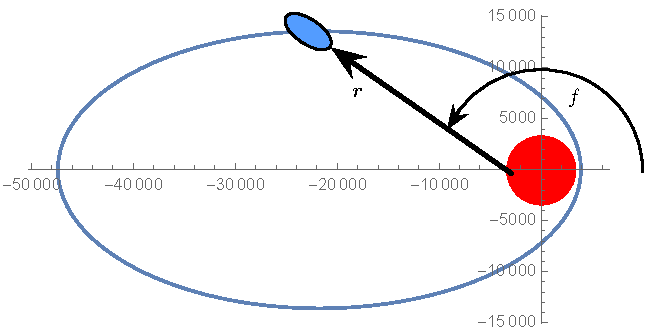
\includegraphics[]{Figures/Fig1}
	}
	\caption{Sample Figure Inclusion.}
	\label{fig:Fig1}
\end{figure}

\section{Introduction}
Provide a brief introduction to the material being discussed in this report.  For example, include what the motivation is, maybe provide a supportive figure such as Figure~\ref{fig:Fig1}, reference earlier work if needed in a literature review.


\section{Document ID}
The technical document ID is setup through the module name.  For example, if the module name is ``subModuleTemplate'', then the  {\tt \ModuleName} parameter is set to this name.  The document ID then becomes {\tt AVS-SIM-subModuleTemplate}.  




\section{Report Formatting and Styling}
\subsection{Equations}
Equations are centered with the equation number flush to the right. In the text, these equations should be referenced by name as Eq.~\eqref{eq:ab} or Equation~\eqref{eq:ab} (e.g., not eq.  1, (1), or Equation 1).
\begin{equation}
	\label{eq:ab}
	a = b^{2}
\end{equation}


\subsection{Citation}
The citation of bibliographical references is indicated in the text by superscripted Arabic numerals, preferably at the end of a sentence.  This is the default style included in this report \LaTeX\ class.

References listed at the end of the paper are indicated in the text by a superscript Arabic number. If this causes confusion in mathematics or if a superscript is not appropriate for other reasons, this can be expressed as (Ref.~1).  

\subsection{Figures}
Illustrations are referred to by name in the text as Figure~1, Figure 2, etc., or, Figures 3 and 4 (e.g., not figure 1, Fig. 1, or \emph{Figure} 1). Captions are in title case (miniscule lettering with the first letter of major words majuscule); they are 10-point serif font and centered below the figure as shown in Figure~\ref{fig:xxx}. Each illustration should have a caption unless it is a mere sketch. An explanatory caption of several sentences is permissible. Each included illustration must be called out (mentioned) in the text. Ideally, figures should appear within the text just before they are called out. 

The figure files (PDF preferred) should be stored in a common ``Figure'' sub-folder.  If available, any drawing documents used to create this figure can be stored in a ``Support'' sub-folder.



\subsection{Tables}
Tables are referred to by name in the text as Table 1, or, Tables 2 and 3 (e.g., not table 1, Tbl. 1, or Table 1). The title is centered above the table, as shown in Table~\ref{tab:label}. The minimum number of lines needed for clarity is desired. The table font may be adjusted smaller than the body text as necessary.

\begin{table}[htbp]
    \caption{A Caption Goes Here}
   \label{tab:label}
        \centering \fontsize{10}{10}\selectfont
   \begin{tabular}{c | r | r } % Column formatting, 
      \hline 
      Animal    & Description & Price (\$)\\
      \hline 
      Gnat      & per gram & 13.65 \\
                & each     &  0.01 \\
      Gnu       & stuffed  & 92.50 \\
      Emu       & stuffed  & 33.33 \\
      Armadillo & frozen   &  8.99 \\
      \hline
   \end{tabular}
\end{table}



\section{Acknowledgment}
Any acknowledgment which the author or authors wish to make may appear here. 



\section{Notation}
If mathematical symbols require definition, a table of notation should appear here. A footnote near the beginning of the paper where mathematics is introduced should direct attention of the reader to this table.





\end{document}
